% ---------------------------------------------
% Alle Abbildungen 'images/' in Latex speichern 
%     * 'archiv/Pics-files.tex' 
%     * Bildgröße: 0.80/1 
% ju 16-Dez-2022 Pics-files.tex
% ---------------------------------------------
%
%\section{01_Generatorregel_Skizze}
%
%01_Generatorregel_Skizze (\autoref{fig:01_Generatorregel_Skizze}).% Referenz
%
\begin{figure}[!hb]% hier: !hb
    \centering
  \includegraphics[width=.80\textwidth]{images/01_Generatorregel_Skizze.pdf}%
  \caption{01_Generatorregel_Skizze}%\label{fig:01_Generatorregel_Skizze}%% anpassen
\end{figure}

%\newpage
%\section{01_Schaltung_Messen_Skizze}
%
%01_Schaltung_Messen_Skizze (\autoref{fig:01_Schaltung_Messen_Skizze}).% Referenz
%
\begin{figure}[!hb]% hier: !hb
    \centering
  \includegraphics[width=.80\textwidth]{images/01_Schaltung_Messen_Skizze.pdf}%
  \caption{01_Schaltung_Messen_Skizze}%\label{fig:01_Schaltung_Messen_Skizze}%% anpassen
\end{figure}

%\newpage
%\section{02_Motorregel_Skizze}
%
%02_Motorregel_Skizze (\autoref{fig:02_Motorregel_Skizze}).% Referenz
%
\begin{figure}[!hb]% hier: !hb
    \centering
  \includegraphics[width=.80\textwidth]{images/02_Motorregel_Skizze.pdf}%
  \caption{02_Motorregel_Skizze}%\label{fig:02_Motorregel_Skizze}%% anpassen
\end{figure}

%\newpage
%\section{02_Schaltung_Messen_Skizze}
%
%02_Schaltung_Messen_Skizze (\autoref{fig:02_Schaltung_Messen_Skizze}).% Referenz
%
\begin{figure}[!hb]% hier: !hb
    \centering
  \includegraphics[width=.80\textwidth]{images/02_Schaltung_Messen_Skizze.pdf}%
  \caption{02_Schaltung_Messen_Skizze}%\label{fig:02_Schaltung_Messen_Skizze}%% anpassen
\end{figure}

%\newpage
%\section{03_Schaltung_Messen_Skizze}
%
%03_Schaltung_Messen_Skizze (\autoref{fig:03_Schaltung_Messen_Skizze}).% Referenz
%
\begin{figure}[!hb]% hier: !hb
    \centering
  \includegraphics[width=.80\textwidth]{images/03_Schaltung_Messen_Skizze.pdf}%
  \caption{03_Schaltung_Messen_Skizze}%\label{fig:03_Schaltung_Messen_Skizze}%% anpassen
\end{figure}

%\newpage
%\section{03_StromdurchflosseneSpule_Skizze}
%
%03_StromdurchflosseneSpule_Skizze (\autoref{fig:03_StromdurchflosseneSpule_Skizze}).% Referenz
%
\begin{figure}[!hb]% hier: !hb
    \centering
  \includegraphics[width=.80\textwidth]{images/03_StromdurchflosseneSpule_Skizze.pdf}%
  \caption{03_StromdurchflosseneSpule_Skizze}%\label{fig:03_StromdurchflosseneSpule_Skizze}%% anpassen
\end{figure}

%\newpage
%\section{04_Stromdichte_Skizze}
%
%04_Stromdichte_Skizze (\autoref{fig:04_Stromdichte_Skizze}).% Referenz
%
\begin{figure}[!hb]% hier: !hb
    \centering
  \includegraphics[width=.80\textwidth]{images/04_Stromdichte_Skizze.pdf}%
  \caption{04_Stromdichte_Skizze}%\label{fig:04_Stromdichte_Skizze}%% anpassen
\end{figure}

%\newpage
%\section{05_StromdurchflossenerLeiter_Skizze}
%
%05_StromdurchflossenerLeiter_Skizze (\autoref{fig:05_StromdurchflossenerLeiter_Skizze}).% Referenz
%
\begin{figure}[!hb]% hier: !hb
    \centering
  \includegraphics[width=.80\textwidth]{images/05_StromdurchflossenerLeiter_Skizze.pdf}%
  \caption{05_StromdurchflossenerLeiter_Skizze}%\label{fig:05_StromdurchflossenerLeiter_Skizze}%% anpassen
\end{figure}

%\newpage
%\section{06_Stromfluss_Messen_Skizze}
%
%06_Stromfluss_Messen_Skizze (\autoref{fig:06_Stromfluss_Messen_Skizze}).% Referenz
%
\begin{figure}[!hb]% hier: !hb
    \centering
  \includegraphics[width=.80\textwidth]{images/06_Stromfluss_Messen_Skizze.pdf}%
  \caption{06_Stromfluss_Messen_Skizze}%\label{fig:06_Stromfluss_Messen_Skizze}%% anpassen
\end{figure}

%\newpage
%\section{07_Reihenschaltung_Widerstaende_Skizze}
%
%07_Reihenschaltung_Widerstaende_Skizze (\autoref{fig:07_Reihenschaltung_Widerstaende_Skizze}).% Referenz
%
\begin{figure}[!hb]% hier: !hb
    \centering
  \includegraphics[width=.80\textwidth]{images/07_Reihenschaltung_Widerstaende_Skizze.pdf}%
  \caption{07_Reihenschaltung_Widerstaende_Skizze}%\label{fig:07_Reihenschaltung_Widerstaende_Skizze}%% anpassen
\end{figure}

%\newpage
%\section{08_Relais_Skizze}
%
%08_Relais_Skizze (\autoref{fig:08_Relais_Skizze}).% Referenz
%
\begin{figure}[!hb]% hier: !hb
    \centering
  \includegraphics[width=.80\textwidth]{images/08_Relais_Skizze.pdf}%
  \caption{08_Relais_Skizze}%\label{fig:08_Relais_Skizze}%% anpassen
\end{figure}

%\newpage
%\section{09_Stroeme_einer_Relaisschaltung_Skizze}
%
%09_Stroeme_einer_Relaisschaltung_Skizze (\autoref{fig:09_Stroeme_einer_Relaisschaltung_Skizze}).% Referenz
%
\begin{figure}[!hb]% hier: !hb
    \centering
  \includegraphics[width=.80\textwidth]{images/09_Stroeme_einer_Relaisschaltung_Skizze.pdf}%
  \caption{09_Stroeme_einer_Relaisschaltung_Skizze}%\label{fig:09_Stroeme_einer_Relaisschaltung_Skizze}%% anpassen
\end{figure}

%\newpage
%\section{10_Stromrelais_Skizze}
%
%10_Stromrelais_Skizze (\autoref{fig:10_Stromrelais_Skizze}).% Referenz
%
\begin{figure}[!hb]% hier: !hb
    \centering
  \includegraphics[width=.80\textwidth]{images/10_Stromrelais_Skizze.pdf}%
  \caption{10_Stromrelais_Skizze}%\label{fig:10_Stromrelais_Skizze}%% anpassen
\end{figure}

%\newpage
%\section{11_Schrittrelais_Skizze}
%
%11_Schrittrelais_Skizze (\autoref{fig:11_Schrittrelais_Skizze}).% Referenz
%
\begin{figure}[!hb]% hier: !hb
    \centering
  \includegraphics[width=.80\textwidth]{images/11_Schrittrelais_Skizze.pdf}%
  \caption{11_Schrittrelais_Skizze}%\label{fig:11_Schrittrelais_Skizze}%% anpassen
\end{figure}

%\newpage
%\section{12_Reedkontaktschalter_Skizze}
%
%12_Reedkontaktschalter_Skizze (\autoref{fig:12_Reedkontaktschalter_Skizze}).% Referenz
%
\begin{figure}[!hb]% hier: !hb
    \centering
  \includegraphics[width=.80\textwidth]{images/12_Reedkontaktschalter_Skizze.pdf}%
  \caption{12_Reedkontaktschalter_Skizze}%\label{fig:12_Reedkontaktschalter_Skizze}%% anpassen
\end{figure}

%\newpage
%\section{13_Spannungsverlust_Skizze}
%
%13_Spannungsverlust_Skizze (\autoref{fig:13_Spannungsverlust_Skizze}).% Referenz
%
\begin{figure}[!hb]% hier: !hb
    \centering
  \includegraphics[width=.80\textwidth]{images/13_Spannungsverlust_Skizze.pdf}%
  \caption{13_Spannungsverlust_Skizze}%\label{fig:13_Spannungsverlust_Skizze}%% anpassen
\end{figure}

%\newpage
%\section{14_ Innenwiderstand_von_Spannungsquellen_Skizze}
%
%14_ Innenwiderstand_von_Spannungsquellen_Skizze (\autoref{fig:14_ Innenwiderstand_von_Spannungsquellen_Skizze}).% Referenz
%
\begin{figure}[!hb]% hier: !hb
    \centering
  \includegraphics[width=.80\textwidth]{images/14_ Innenwiderstand_von_Spannungsquellen_Skizze.pdf}%
  \caption{14_ Innenwiderstand_von_Spannungsquellen_Skizze}%\label{fig:14_ Innenwiderstand_von_Spannungsquellen_Skizze}%% anpassen
\end{figure}

%\newpage
%\section{15_Schaltzeichen_Widerstand_Skizze}
%
%15_Schaltzeichen_Widerstand_Skizze (\autoref{fig:15_Schaltzeichen_Widerstand_Skizze}).% Referenz
%
\begin{figure}[!hb]% hier: !hb
    \centering
  \includegraphics[width=.80\textwidth]{images/15_Schaltzeichen_Widerstand_Skizze.pdf}%
  \caption{15_Schaltzeichen_Widerstand_Skizze}%\label{fig:15_Schaltzeichen_Widerstand_Skizze}%% anpassen
\end{figure}

%\newpage
%\section{16_Widerstandsmessung_Skizze}
%
%16_Widerstandsmessung_Skizze (\autoref{fig:16_Widerstandsmessung_Skizze}).% Referenz
%
\begin{figure}[!hb]% hier: !hb
    \centering
  \includegraphics[width=.80\textwidth]{images/16_Widerstandsmessung_Skizze.pdf}%
  \caption{16_Widerstandsmessung_Skizze}%\label{fig:16_Widerstandsmessung_Skizze}%% anpassen
\end{figure}

%\newpage
%\section{17_Leistungsteilung_Skizze}
%
%17_Leistungsteilung_Skizze (\autoref{fig:17_Leistungsteilung_Skizze}).% Referenz
%
\begin{figure}[!hb]% hier: !hb
    \centering
  \includegraphics[width=.80\textwidth]{images/17_Leistungsteilung_Skizze.pdf}%
  \caption{17_Leistungsteilung_Skizze}%\label{fig:17_Leistungsteilung_Skizze}%% anpassen
\end{figure}

%\newpage
%\section{18_Stromflusserhoehung_Strombegrenzung_Spannungsteilung_Skizze}
%
%18_Stromflusserhoehung_Strombegrenzung_Spannungsteilung_Skizze (\autoref{fig:18_Stromflusserhoehung_Strombegrenzung_Spannungsteilung_Skizze}).% Referenz
%
\begin{figure}[!hb]% hier: !hb
    \centering
  \includegraphics[width=.80\textwidth]{images/18_Stromflusserhoehung_Strombegrenzung_Spannungsteilung_Skizze.pdf}%
  \caption{18_Stromflusserhoehung_Strombegrenzung_Spannungsteilung_Skizze}%\label{fig:18_Stromflusserhoehung_Strombegrenzung_Spannungsteilung_Skizze}%% anpassen
\end{figure}

%\newpage
%\section{19_Parallelschaltung_Widerstaende_Skizze}
%
%19_Parallelschaltung_Widerstaende_Skizze (\autoref{fig:19_Parallelschaltung_Widerstaende_Skizze}).% Referenz
%
\begin{figure}[!hb]% hier: !hb
    \centering
  \includegraphics[width=.80\textwidth]{images/19_Parallelschaltung_Widerstaende_Skizze.pdf}%
  \caption{19_Parallelschaltung_Widerstaende_Skizze}%\label{fig:19_Parallelschaltung_Widerstaende_Skizze}%% anpassen
\end{figure}

%\newpage
%\section{28_FT_Brueckenschaltung}
%
%28_FT_Brueckenschaltung (\autoref{fig:28_FT_Brueckenschaltung}).% Referenz
%
\begin{figure}[!hb]% hier: !hb
    \centering
  \includegraphics[width=.80\textwidth]{images/28_FT_Brueckenschaltung.pdf}%
  \caption{28_FT_Brueckenschaltung}%\label{fig:28_FT_Brueckenschaltung}%% anpassen
\end{figure}

%\newpage
%\section{28_FT_Potentialbestimmung}
%
%28_FT_Potentialbestimmung (\autoref{fig:28_FT_Potentialbestimmung}).% Referenz
%
\begin{figure}[!hb]% hier: !hb
    \centering
  \includegraphics[width=.80\textwidth]{images/28_FT_Potentialbestimmung.pdf}%
  \caption{28_FT_Potentialbestimmung}%\label{fig:28_FT_Potentialbestimmung}%% anpassen
\end{figure}

%\newpage
%\section{Messmethodik_Schaltkreis}
%
%Messmethodik_Schaltkreis (\autoref{fig:Messmethodik_Schaltkreis}).% Referenz
%
\begin{figure}[!hb]% hier: !hb
    \centering
  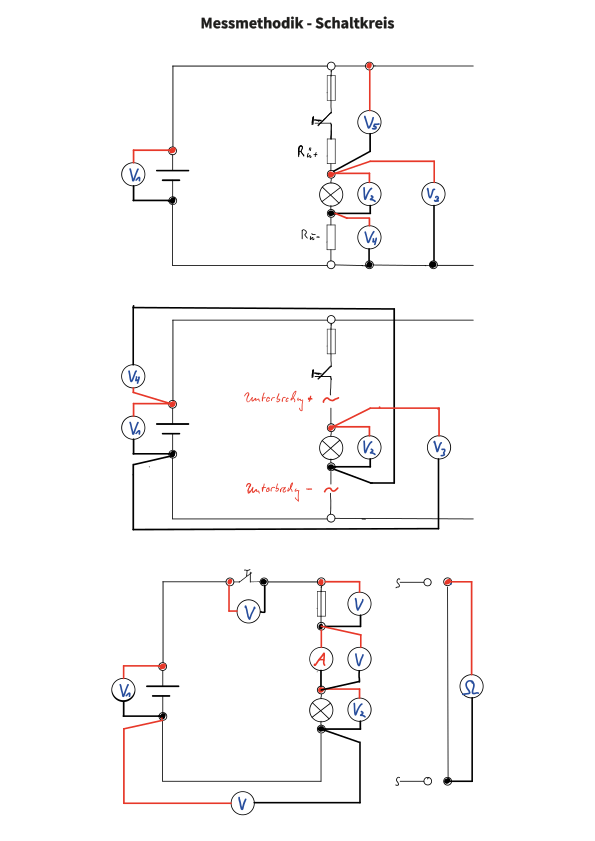
\includegraphics[width=.80\textwidth]{images/Messmethodik_Schaltkreis.pdf}%
  \caption{Messmethodik_Schaltkreis}%\label{fig:Messmethodik_Schaltkreis}%% anpassen
\end{figure}

%\newpage
